\documentclass[twoside]{article}
\usepackage{amsmath}
\usepackage{amssymb}
\usepackage{amsthm}
\usepackage{calc}
\usepackage{capt-of}
\usepackage{caption}
\usepackage[strict]{changepage}
\usepackage{chngcntr}
\usepackage[americanvoltage,siunitx]{circuitikz}
\usepackage{color,colortbl}
\usepackage{etoolbox}
\usepackage{fancyhdr}
\usepackage[T1]{fontenc}
\usepackage{gensymb}
\usepackage[margin=1in]{geometry}
\usepackage{graphicx}
\usepackage{hyperref}
\usepackage{import}
\usepackage{indentfirst}
\usepackage{mathptmx}
\usepackage{mathrsfs}
\usepackage{multicol}
\usepackage{multirow}
\usepackage{needspace}
\usepackage{pgfplots}
\usepackage{pgfplotstable}
\usepackage{setspace}
\usepackage{siunitx}
\usepackage{tabu}
\usepackage{tabularx}
\usepackage{tikz}
\usepackage{xspace}

\patchcmd{\thebibliography}{\section*{\refname}}{\vspace{-1em}}{}{}

\captionsetup{labelformat=empty,labelsep=none}
\usepgfplotslibrary{external}
\usetikzlibrary{positioning,matrix,shapes,chains,arrows}
\tikzexternalize[prefix=precompiled_figures/]

\newcommand\svgsize[2]{\def\svgwidth{#2}
{\centering\input{#1.pdf_tex}}}
\newcommand\svgc[1]{\svgsize{#1}{\columnwidth}}
\newcommand\svgl[1]{\svgsize{#1}{1em}}
\newcommand\diagrams[0]{\renewcommand\svgsize[2]{\def\svgwidth{##2}
{\centering\input{diagrams/##1.pdf_tex}}}}

\newcommand\pdf[1]{\noindent\includegraphics[width=\columnwidth]{#1.pdf}}
\newcommand\pdfex[1]{\pdf{#1}

\pdf{#1ex}}
\newcommand\pdfmsg[1]{\noindent\begin{minipage}{\columnwidth}\pdf{#1msg}

\pdf{#1}\end{minipage}}
\newcommand\pdfmsgex[1]{\pdfmsg{#1}

\pdf{#1ex}}
\newcommand\code[0]{\renewcommand\pdf[1]{\noindent
\includegraphics[width=\columnwidth]{code/##1.pdf}}}

% Indent
\setlength{\parindent}{0.3in}

\newcounter{paperthmamount}
\newcommand\theorems[0]{
\theoremstyle{remark}
\newtheorem{claim}[subsection]{Claim}
\theoremstyle{plain}
\newtheorem{conjecture}[subsection]{Conjecture}
\theoremstyle{plain}
\newtheorem{corollary}[subsection]{Corollary}
\theoremstyle{definition}
\newtheorem{definition}[subsection]{Definition}
\theoremstyle{plain}
\newtheorem{lemma}[subsection]{Lemma}
\theoremstyle{remark}
\newtheorem{proposition}[subsection]{Proposition}
\theoremstyle{remark}
\newtheorem{remark}[subsection]{Remark}
\theoremstyle{plain}
\newtheorem{theorem}[subsection]{Theorem}
\theoremstyle{definition}
\newtheorem{question}[subsection]{Question}
\newcommand\paperclm[2]
{\begin{claim}\global\expandafter\edef
\csname clm##1\endcsname{Claim \thesubsection\noexpand\xspace}
##2\end{claim}}
\newcommand\papercnj[2]
{\begin{conjecture}\global\expandafter\edef
\csname cnj##1\endcsname{Conjecture \thesubsection\noexpand\xspace}
##2\end{conjecture}}
\newcommand\papercor[2]
{\begin{corollary}\global\expandafter\edef
\csname cor##1\endcsname{Corollary \thesubsection\noexpand\xspace}
##2\end{corollary}}
\newcommand\paperdef[2]
{\begin{definition}\global\expandafter\edef
\csname def##1\endcsname{Definition \thesubsection\noexpand\xspace}
##2\end{definition}}
\newcommand\paperlem[2]
{\begin{lemma}\global\expandafter\edef
\csname lem##1\endcsname{Lemma \thesubsection\noexpand\xspace}
##2\end{lemma}}
\newcommand\paperprp[2]
{\begin{proposition}\global\expandafter\edef
\csname prp##1\endcsname{Proposition \thesubsection\noexpand\xspace}
##2\end{proposition}}
\newcommand\paperqtn[2]
{\begin{question}\global\expandafter\edef
\csname qtn##1\endcsname{Question \thesubsection\noexpand\xspace}
##2\end{question}}
\newcommand\paperrem[2]
{\begin{remark}\global\expandafter\edef
\csname rem##1\endcsname{Remark \thesubsection\noexpand\xspace}
##2\end{remark}}
\newcommand\paperthm[2]
{\begin{theorem}\global\expandafter\edef
\csname thm##1\endcsname{Theorem \thesubsection\noexpand\xspace}
##2\end{theorem}}}
\newcommand\subtheorems[0]{\stepcounter{paperthmamount}
\theoremstyle{remark}
\newtheorem{claim}[subsubsection]{Claim}
\theoremstyle{plain}
\newtheorem{conjecture}[subsubsection]{Conjecture}
\theoremstyle{plain}
\newtheorem{corollary}[subsubsection]{Corollary}
\theoremstyle{definition}
\newtheorem{definition}[subsubsection]{Definition}
\theoremstyle{plain}
\newtheorem{lemma}[subsubsection]{Lemma}
\theoremstyle{remark}
\newtheorem{proposition}[subsubsection]{Proposition}
\theoremstyle{remark}
\newtheorem{remark}[subsubsection]{Remark}
\theoremstyle{plain}
\newtheorem{theorem}[subsubsection]{Theorem}
\theoremstyle{definition}
\newtheorem{question}[subsubsection]{Question}
\newcommand\paperclm[2]
{\begin{claim}\global\expandafter\edef
\csname clm##1\endcsname{Claim \thesubsubsection\noexpand\xspace}
##2\end{claim}}
\newcommand\papercnj[2]
{\begin{conjecture}\global\expandafter\edef
\csname cnj##1\endcsname{Conjecture \thesubsubsection\noexpand\xspace}
##2\end{conjecture}}
\newcommand\papercor[2]
{\begin{corollary}\global\expandafter\edef
\csname cor##1\endcsname{Corollary \thesubsubsection\noexpand\xspace}
##2\end{corollary}}
\newcommand\paperdef[2]
{\begin{definition}\global\expandafter\edef
\csname def##1\endcsname{Definition \thesubsubsection\noexpand\xspace}
##2\end{definition}}
\newcommand\paperlem[2]
{\begin{lemma}\global\expandafter\edef
\csname lem##1\endcsname{Lemma \thesubsubsection\noexpand\xspace}
##2\end{lemma}}
\newcommand\paperprp[2]
{\begin{proposition}\global\expandafter\edef
\csname prp##1\endcsname{Proposition \thesubsubsection\noexpand\xspace}
##2\end{proposition}}
\newcommand\paperqtn[2]
{\begin{question}\global\expandafter\edef
\csname qtn##1\endcsname{Question \thesubsubsection\noexpand\xspace}
##2\end{question}}
\newcommand\paperrem[2]
{\begin{remark}\global\expandafter\edef
\csname rem##1\endcsname{Remark \thesubsubsection\noexpand\xspace}
##2\end{remark}}
\newcommand\paperthm[2]
{\begin{theorem}\global\expandafter\edef
\csname thm##1\endcsname{Theorem \thesubsubsection\noexpand\xspace}
##2\end{theorem}}}

% Title section
\pagestyle{fancy}
\thispagestyle{empty}
\renewcommand{\headrulewidth}{0pt}
\newcommand\papertitle[1]
{{\centering\fontsize{20pt}{20pt}\textsc{#1}\\\mbox{}\\}
\fancyhead[OC]{\fontsize{12pt}{12pt}\selectfont\textit{#1}}}
\newcounter{people}
\newcommand\paperauthtext[3]{{\centering\fontsize{12pt}{12pt}\selectfont
\textsc{#1}\\[-0.1em]{\fontsize{9pt}{9pt}\selectfont\textit{\ifx&#2&
\vspace{-1em}\else#2\fi}}\\\mbox{}\\
\fancyhead[EC]{\fontsize{12pt}{12pt}\selectfont\textit{#3}}}}
\newcommand\paperauth[2]{{\stepcounter{people}
\ifnum\value{people}=1
{\paperauthtext{#1}{#2}{#1}
\global\def\auth{#1\xspace}}
\else\ifnum\value{people}=2
{\paperauthtext{#1}{#2}{\auth and #1}}
\else{\paperauthtext{#1}{#2}{\auth et al}}\fi\fi}}
\newcommand\physics[0]{
\renewcommand\paperauthtext[4]{{\centering\fontsize{12pt}{12pt}\selectfont
\textsc{##1. ##2}\\[-0.1em]{\fontsize{9pt}{9pt}\selectfont\textit{\ifx&##3&
\vspace{-1em}\else##3\fi}}\\\mbox{}\\
\fancyhead[EC]{\fontsize{12pt}{12pt}\selectfont\textit{##4}}}}
\renewcommand\paperauth[3]{{\stepcounter{people}
\ifnum\value{people}=1
{\paperauthtext{##1}{##2}{##3}{##1. ##2}
\global\def\auth{##2\xspace}}
\else\ifnum\value{people}=2
{\paperauthtext{##1}{##2}{##3}{\auth and ##2}}
\else{\paperauthtext{##1}{##2}{##3}{\auth et al}}\fi\fi}}}
\newcommand\paperdate[1]{{\centering\fontsize{9pt}{9pt}\selectfont\text{
(Received #1)}\\[2em]}}

% Page header
\newcommand{\paperhead}[1]{\fancyhead[EC]{\fontsize{12pt}{12pt}\selectfont
\textit{#1}}}
\fancyhead[RO, EL]{\fontsize{12pt}{12pt}\selectfont\thepage}
\fancyhead[RE, OL]{}
\cfoot{}

\makeatletter
\newenvironment{paperadjustwidth}[2]{
  \begin{list}{}{
    \setlength\partopsep\z@
    \setlength\topsep\z@
    \setlength\listparindent\parindent
    \setlength\parsep\parskip
    \@ifmtarg{#1}{\setlength{\leftmargin}{\z@}}
                 {\setlength{\leftmargin}{#1}}
    \@ifmtarg{#2}{\setlength{\rightmargin}{\z@}}
                 {\setlength{\rightmargin}{#2}}
    }
    \item[]}{\end{list}}
\makeatother

%Figure counter
\newcounter{paperfigurecounter}
\newcommand{\papercap}[2]{\bgroup\stepcounter{paperfigurecounter}
\captionof{figure}{\fontsize{9pt}{9pt}\selectfont
\hspace{0.3in}Fig.~\arabic{paperfigurecounter}.\quad#2}
\egroup\expandafter\edef
\csname fig#1\endcsname{Fig.~\arabic{paperfigurecounter}\noexpand\xspace}}

\newcommand\paperfig[3]{\noindent\begin{minipage}{\columnwidth}
#2\papercap{#1}{#3}\end{minipage}\expandafter\edef
\csname fig#1\endcsname{Fig.~\arabic{paperfigurecounter}\noexpand\xspace}}
\newcommand\papersvg[3]{\paperfig{#1}{\svgc{#2}}{#3}}

% Abstract environment
\newenvironment{paperabs}
{\begin{paperadjustwidth}{0.5in}{0.5in}\bgroup\fontsize{9pt}{9pt}\selectfont
\hspace{0.5in}}
{\egroup\end{paperadjustwidth}}

% Paper environment
\setlength\columnsep{0.5in}
\newenvironment{paper}
{\begin{multicols*}{2}\bgroup\fontsize{12pt}{12pt}\selectfont}
{\egroup\end{multicols*}}
\newcommand{\singlecolumn}[0]{
\renewcommand\paperfig[3]{\noindent
\makebox[\textwidth][c]{\begin{minipage}{5.5in}
\noindent\makebox[\textwidth][c]{\begin{minipage}{3in}##2\end{minipage}}
\papercap{##1}{##3}\end{minipage}}\expandafter\edef
\csname fig##1\endcsname{Fig.~\arabic{paperfigurecounter}\noexpand\xspace}}
\renewenvironment{paper}{\bgroup\fontsize{12pt}{12pt}\selectfont}
{\egroup}}

%Sources
\newsavebox{\sourcebox}
\newcommand{\papersource}[1]{
\vspace{-2em}
\text{}\\*
\fontsize{9pt}{9pt}\selectfont
\noindent\renewcommand{\labelenumi}{}
\savebox{\sourcebox}{\parbox{3in}{\begin{enumerate}
\setlength{\leftmargini}{-1ex}
\setlength{\leftmargin}{-1ex}
\setlength{\labelwidth}{0pt}
\setlength{\labelsep}{0pt}
\setlength{\listparindent}{0pt}
\item\textit{\hspace{-0.35in}#1}
\end{enumerate}}}
\usebox{\sourcebox}
}

%Section headers
\newcounter{paperseccounter}
\newcounter{papersubseccounter}[paperseccounter]
\newcommand\papersec[1]{\needspace{1in}
\stepcounter{paperseccounter}
\stepcounter{section}
\begin{center}\Roman{paperseccounter} \textsc{#1}\end{center}}
\newcommand\papersubsec[1]{\needspace{1in}
\stepcounter{papersubseccounter}
\addtocounter{subsection}{\thepaperthmamount}
\setcounter{subsubsection}{0}
{\begin{center}
\Roman{section}.\Roman{papersubseccounter}
\textsc{#1}\\[0.5em]\end{center}}}

%equation
\newcounter{papereqcounter}
\newcommand\papereq[3]{{
\stepcounter{papereqcounter}
\mbox{}\vspace{-0.75em}
\begin{equation*}
#2
\tag*{\fontsize{12pt}{12pt}\selectfont
$\begin{array}{r}
\cr{\text{(\arabic{papereqcounter})}}
\cr{\fontsize{9pt}{9pt}\selectfont\textit{\ifx\\#3\\~\else(\fi#3\ifx\\#3\\~
\else)\fi}}
\end{array}$}
\end{equation*}

}
\expandafter\edef\csname eq#1\endcsname{(\arabic{papereqcounter})\noexpand
\xspace}}

% Where
\newcommand{\papervar}[3]
{&$#1$ & #2 \ifx\\#3\\~\else($\smash{\text{\si{\fi
#3\ifx\\#3\\~\else}}}$)\fi\\}
\newenvironment{paperwhere}
{\begin{minipage}{\columnwidth}
\bgroup\fontsize{9pt}{9pt}\selectfont Where:\vspace{2pt}\\\begin{tabular}
{rr@{ = }p{\linewidth}}}
{\end{tabular}\egroup\end{minipage}\vspace{5pt}}

% Tables
\definecolor{LineGray}{gray}{0.5}
\newtabulinestyle{outer=2.25pt LineGray}
\newtabulinestyle{inner=0.75pt LineGray}
\tabulinesep=1.5pt

\newcommand{\paperiline}[0]{\tabucline[inner]{-}}
\newcommand{\paperoline}[0]{\tabucline[outer]{-}}

% Index column type
\newcolumntype{I}{X[-5,c]}
% Column type with uncertainty
\newcolumntype{U}{@{}X[-5,r]@{$\pm$}X[-5,l]@{}}
% Column type without uncertainty
\newcolumntype{C}{@{}X[-5,c]@{}}

\newcounter{papertableindexcounter}
\newcommand{\papertableindexheader}[0]{\multirow{2}{*}{\textsc{Index}}}
\newcommand{\papertableindex}[0]{\stepcounter{papertableindexcounter}
\arabic{papertableindexcounter}}
\newcommand{\papertableuheadersymbol}[1]{&\multicolumn{2}{c|[inner]}{$#1$}}
\newcommand{\papertableuheadersymbole}[1]{&\multicolumn{2}{c|[outer]}{$#1$}}
\newcommand{\papertableuheaderunit}[1]{&\multicolumn{2}{c|[inner]}{(#1)}}
\newcommand{\papertableuheaderunite}[1]{&\multicolumn{2}{c|[outer]}{(#1)}}
\newcommand{\papertablecheadersymbol}[1]{&$#1$}
\newcommand{\papertablecheaderunit}[2]{&($\pm$#1 #2)}

% Value in table with uncertainty.
\newcommand{\papertableuval}[2]{& #1 & #2}
% Value in table without uncertainty.
\newcommand{\papertablecval}[1]{& #1}

\newenvironment{papertable}[1]
{\setcounter{papertableindexcounter}{0} 
\begin{tabu} to \linewidth {#1}}
{\end{tabu}\vspace{12pt}}

\newcommand{\paperaxis}[9]
{title=#1,
axis x line = bottom,
xmin=#4,xmax=#6,
axis y line = left,
ymin=#5,ymax=#7,
height = 180pt,
grid=both,
x axis line style=-,
y axis line style=-,
x tick label style={
/pgf/number format/.cd,
fixed,
fixed zerofill,
precision=#8,
/tikz/.cd},
y tick label style={
/pgf/number format/.cd,
fixed,
fixed zerofill,
precision=#9,
/tikz/.cd}}
\newcommand{\paperaxisxlabel}[2]{
xlabel=\fontsize{10pt}{10pt}\selectfont#1$(#2)\rightarrow$}
\newcommand{\paperaxisylabel}[2]{
ylabel=\fontsize{10pt}{10pt}\selectfont#1$(#2)\rightarrow$}
\newcommand{\papergraphoutline}[4]{
\addplot [mark=none,line width=0.75pt] coordinates {
(#1,#2)
(#1,#4)
(#3,#4)
(#3,#2)
(#1,#2)};}

\newenvironment{papergraph}{
\begin{tikzpicture}
\begin{axis}}
{\end{axis}
\end{tikzpicture}}

\newcommand{\comment}[1]{}

\newcommand{\abs}[1]{\left\lvert#1\right\rvert}
\newcommand{\oo}[0]{\infty}
\newcommand{\sigmaSum}[3]{\sum\limits_{#1}^{#2} #3}
\newcommand{\limto}[3]{\lim\limits_{#1\rightarrow#2}#3}
\renewcommand{\d}[0]{\mathrm{d}}
\newcommand{\cross}[0]{\times}
\newcommand{\lp}{\left(}
\newcommand{\rp}{\right)}
\newcommand\pars[1]{\lp#1\rp}
\newcommand\sqbrack[1]{\left[#1\right]}
\newcommand\R{\mathbb{R}}
\newcommand\di{\partial}
\newcommand\x{\times}
\newcommand\del{\nabla}

<<<<<<< HEAD
\usepackage{tikz}
\usetikzlibrary{optics}

\usepackage{verbatim}

=======
>>>>>>> bdd2129682700780a43f68eb3971bc92bf39636a
\physics
\begin{document}
\papertitle{Two-Terminal Devices}
\paperauth{A}{Khesin}{1002442029}
\paperauth{P}{Zavyalova}{1002345036}
\paperdate{March 19, 2018, Completed March 13, 2018}
\begin{paperabs}

	Abstract goes here
	
\end{paperabs}

\begin{paper}
	
\papersec{Introduction}
	
<<<<<<< HEAD
	The operation of a two-terminal device may be completely described by providing a relationship between the current through the device and the voltage across it. In this lab, the latter relation was determined for a variety of circuit elements, including resistors, a resistor in series with a dry cell, several diodes, a thermistor, and a section of a rectifier. 
	
	\textbf{TODO}: circuit diagram + description.
	
	Prior to wiring the circuit as displayed above, vertical and horizontal sensitivities of the oscilloscope along with its zeros were set. The desired I vs. V curves were displayed in the Y vs. X mode of the oscilloscope; to obtain current as opposed to potential on the dependent axes, the Y voltage was divided by \( R_2 = 4.7 \si{\ohm} \) before plotting. The final experimental setup looked as shown below.
	
	\paperfig{SetupMain}{\pdf{setup_main}}{Experimental setup used to determine I vs. V plots for a variety of provided circuit components, with the diode vacuum tube specifically investigated here.}
	
	To further interpret the obtained I vs. V curves, a multimeter was used to measure the resistance of each component, with the connections made in both possible directions. 
	
	Additionally, I vs. V graphs of several capacitors, inductors, and a potentiometer were obtained. The same circuit as in \textbf{TODO} was used, resulting in the following setup.
	
	\paperfig{SetupAdditional}{\pdf{setup_additional}}{Experimental setup used to determine I vs. V curves of additional circuit components, with a \( 100 \si{\kilo\ohm} \) connected here.}
	
=======
	Introduction goes here

\paperfig{Circuit}{\begin{center}
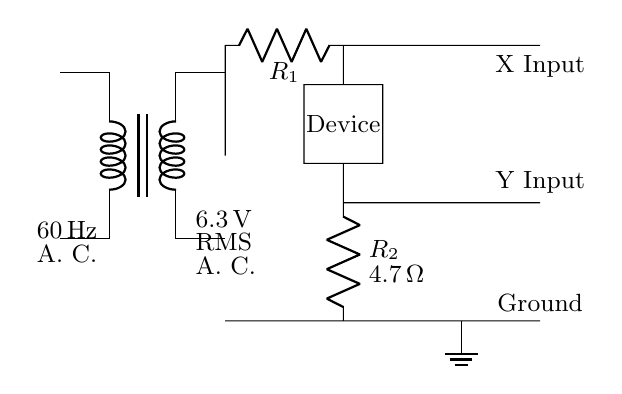
\begin{tikzpicture}
\draw
(2,2) rectangle (3,3)
(2.5,2) |- (5,1.5)
(2.5,1.5) to[resistor] (2.5,0)
(1,0) -- (5,0)
(2.5,3) |- (5,3.5)
(2.5,3.5) to[resistor] (1,3.5) -- (1,2.1)
(-0.05,2.1) node[transformer core]{}
(4,0) node[ground]{}
(5,0) node[above]{\small Ground}
(5,1.5) node[above]{\small Y Input}
(5,3.5) node[below]{\small X Input}
(2.5,2.5) node[]{\small Device}
(2.7,0.9) node[right]{\small $R_2$}
(2.7,0.6) node[right]{\small\SI{4.7}{\ohm}}
(1.75,3.4) node[below]{\small $R_1$}
(0.5,1.3) node[right]{\small \SI{6.3}{\volt}}
(0.5,1) node[right]{\small RMS}
(0.5,0.7) node[right]{\small A. C.}
(-0.5,0.85) node[left]{\small A. C.}
(-0.5,1.15) node[left]{\small \SI{60}{\hertz}}
;
\end{tikzpicture}\end{center}}
{The circuit used in the experiment.
The value of $R_1$ was varied depending on what was used for the Device.
The $X$ and $Y$ nodes were connected to an oscilloscope.}

>>>>>>> bdd2129682700780a43f68eb3971bc92bf39636a
\papersec{Observations}
	
	To obtain I vs. V plots for the circuit components investigated, measurements were first saved using the \textit{Save} function of the oscilloscope. Dividing the channel two voltage by the resistance as described above, the desired plots were obtained.  Note that \( R_1 \) in \textbf{TODO} varied for each circuit component. 
	
	% \begin{comment}
	\paperfig{ShortCircuit}{\pdf{char_curves/1-short}}{I vs. V curve for a short circuit, with \( R_1 \) set to \( 100 \si{\ohm} \).}
	\paperfig{Resistor47}{\pdf{char_curves/2-47}}{I vs. V curve for a \( 47 \si{\ohm} \) resistor, with \( R_1 \) set to \( 100 \si{\ohm} \).}	
	\paperfig{Resistor1000}{\pdf{char_curves/3-1000}}{I vs. V curve for a \( 1000 \si{\ohm} \) resistor, with \( R_1 \) set to \( 100 \si{\ohm} \).}	
	\paperfig{CellUp}{\pdf{char_curves/4a-cell-up}}{I vs. V curve for a \( 47 \si{\ohm} \) resistor in series with a 1 1/2 volt dry cell in the \textbf{positive direction???}. Here, \( R_1 \) of \( 100 \si{\ohm} \) was used.}	
	\paperfig{CellDown}{\pdf{char_curves/4b-cell-down}}{I vs. V curve for a \( 47 \si{\ohm} \) resistor in series with a 1 1/2 volt dry cell in the \textbf{negative direction???}. Here, \( R_1 \) of \( 100 \si{\ohm} \) was used.}
	\paperfig{Germanium}{\pdf{char_curves/5-germanium}}{I vs. V curve for a germanium diode. Here, \( R_1 \) of \( 100 \si{\ohm} \) was used.}
	\paperfig{Silicon}{\pdf{char_curves/6-silicon}}{I vs. V curve for a silicon diode. Here, \( R_1 \) of \( 100 \si{\ohm} \) was used.}
	\paperfig{Selenium}{\pdf{char_curves/7-selenium}}{I vs. V curve for a one section of a selenium rectifier. Here, \( R_1 \) of \( 100 \si{\ohm} \) was used.}
	\paperfig{Vacuum}{\pdf{char_curves/8-vacuum}}{I vs. V curve for a diode vacuum tube. Here, \( R_1 \) of \( 0 \si{\ohm} \) was used.}
	\paperfig{Zener}{\pdf{char_curves/9-zener}}{I vs. V curve for a zener diode. Here, \( R_1 \) of \( 100 \si{\ohm} \) was used.}
	\paperfig{Thermistor}{\pdf{char_curves/10-thermistor}}{I vs. V curve for a thermistor. Here, \( R_1 \) of \( 50 \si{\ohm} \) was used.}
	% \end{comment}
	
	\begin{comment}
	\paperfig{ShortCircuit}{\pdf{char_curves\\1-short}}{I vs. V curve for a short circuit, with \( R_1 \) set to \( 100 \si{\ohm} \).}
	\paperfig{ShortCircuit}{\pdf{char_curves\\2-47}}{I vs. V curve for a \( 47 \si{\ohm} \) resistor, with \( R_1 \) set to \( 100 \si{\ohm} \).}
	\paperfig{Resistor1000}{\pdf{char_curves\\3-1000}}{I vs. V curve for a \( 1000 \si{\ohm} \) resistor, with \( R_1 \) set to \( 100 \si{\ohm} \).}	
	\paperfig{CellUp}{\pdf{char_curves\\4a-cell-up}}{I vs. V curve for a \( 47 \si{\ohm} \) resistor in series with a 1 1/2 volt dry cell in the \textbf{positive direction???}. Here, \( R_1 \) of \( 100 \si{\ohm} \) was used.}
	\paperfig{CellDown}{\pdf{char_curves\\4b-cell-down}}{I vs. V curve for a \( 47 \si{\ohm} \) resistor in series with a 1 1/2 volt dry cell in the \textbf{negative direction???}. Here, \( R_1 \) of \( 100 \si{\ohm} \) was used.}
	\paperfig{Germanium}{\pdf{char_curves\\5-germanium}}{I vs. V curve for a germanium diode. Here, \( R_1 \) of \( 100 \si{\ohm} \) was used.}
	\paperfig{Silicon}{\pdf{char_curves\\6-silicon}}{I vs. V curve for a silicon diode. Here, \( R_1 \) of \( 100 \si{\ohm} \) was used.}
	paperfig{Selenium}{\pdf{char_curves\\7-selenium}}{I vs. V curve for a one section of a selenium rectifier. Here, \( R_1 \) of \( 100 \si{\ohm} \) was used.}
	\paperfig{Vacuum}{\pdf{char_curves\\8-vacuum}}{I vs. V curve for a diode vacuum tube. Here, \( R_1 \) of \( 0 \si{\ohm} \) was used.}
	\paperfig{Zener}{\pdf{char_curves\\9-zener}}{I vs. V curve for a zener diode. Here, \( R_1 \) of \( 100 \si{\ohm} \) was used.}
	\paperfig{Thermistor}{\pdf{char_curves\\10-thermistor}}{I vs. V curve for a thermistor. Here, \( R_1 \) of \( 50 \si{\ohm} \) was used.}
	\end{comment}
	
\paperfig{Resistances}{\begin{papertable}{|[outer]I|[inner]C|[inner]U|[outer]}\paperoline
\papertableindexheader&\multirow{2}{*}{\textsc{Device}}\papertableuheadersymbole{\textsc{Resistance}}\\
&\papertableuheadersymbole{R$ $(\si{\ohm})}\\\paperiline
\papertableindex\papertablecval{Short Circuit}\papertableuval{0.0}{.3}\\\paperiline
\papertableindex\papertablecval{\SI{47}{\ohm} Resistor}\papertableuval{47.0}{.8}\\\paperiline
\papertableindex\papertablecval{\SI{1}{\kilo\ohm} Resistor}\papertableuval{990}{10}\\\paperiline
\papertableindex\papertablecval{With Cell (+/-)}\papertableuval{(5.21}{.04)\SI{E6}{}}\\\paperiline
\papertableindex\papertablecval{Ge (+ Cathode)}\papertableuval{2830}{30}\\\paperiline
\papertableindex\papertablecval{Ge (+ Anode)}\papertableuval{$\infty$}{?}\\\paperiline
\papertableindex\papertablecval{Si (+ Cathode)}\papertableuval{(3.33}{.03)\SI{E6}{}}\\\paperiline
\papertableindex\papertablecval{Si (+ Anode)}\papertableuval{$\infty$}{?}\\\paperiline
\papertableindex\papertablecval{Se (+ Cathode)}\papertableuval{(18.4}{.2)\SI{E3}{}}\\\paperiline
\papertableindex\papertablecval{Se (+ Anode)}\papertableuval{(61.4}{.5)\SI{E3}{}}\\\paperiline
\papertableindex\papertablecval{Tube (+ Cathode)}\papertableuval{7020}{60}\\\paperiline
\papertableindex\papertablecval{Tube (+ Anode)}\papertableuval{$\infty$}{?}\\\paperiline
\papertableindex\papertablecval{Zener (+ Cathode)}\papertableuval{(25.2}{.2)\SI{E6}{}}\\\paperiline
\papertableindex\papertablecval{Zener (+ Anode)}\papertableuval{$\infty$}{?}\\\paperiline
\papertableindex\papertablecval{Thermistor}\papertableuval{1150}{10}\\\paperiline
\papertableindex\papertablecval{\SI{68.6}{\milli\henry} Inductor}\papertableuval{0.3}{.3}\\\paperiline
\papertableindex\papertablecval{\SI{1.68}{\milli\henry} Inductor}\papertableuval{0.0}{.3}\\\paperiline
\papertableindex\papertablecval{\SI{1.0}{\micro\farad} Capacitor}\papertableuval{$\infty$}{?}\\\paperiline
\papertableindex\papertablecval{\SI{22}{\nano\farad} Capacitor}\papertableuval{$\infty$}{?}\\\paperiline
\papertableindex\papertablecval{\SI{0.1}{\micro\farad} Capacitor}\papertableuval{$\infty$}{?}\\\paperiline
\papertableindex\papertablecval{5-\SI{50}{\ohm} Pot.}\papertableuval{5.0}{.3}\\\paperoline
\end{papertable}\vspace{-1.5em}}
{A table of the resistances of various devices used in the experiment.
For each device, the resistance was measured in both directions, if it was found to be the same, it was recorded in a single line,
otherwise, it was recorded with a note indicating if the positive lead of the multimeter was at the cathode or the anode of the device.
In cases where the resistance was so large that it could not be accurately measured by the multimeter, or in the cases where it was oscillating between large and small values and was not stabilising, $(\infty\pm?)$ was recorded.
The entries in the table are for the following devices: a short circuit, a \SI{47}{\ohm} resistor, a \SI{1}{\kilo\ohm} resistor, a \SI{47}{\ohm} resistor in series with a \SI{1.5}{\volt} battery in both directions, a germanium diode, a silicon diode, one section of a selenium rectifier, a diode vacuum tube, a zener diode, a thermistor, a \SI{68.6}{\milli\henry} inductor, a \SI{1.68}{\milli\henry} inductor, a \SI{1.0}{\micro\farad} capacitor, a \SI{22}{\nano\farad} capacitor, a \SI{0.1}{\micro\farad} capacitor, and a a $5-\SI{50}{\ohm}$ potentiometer which was set to its lowest setting.}
	
\papersec{Analysis} 
	
	
	
\papersec{Conclusion}

	Conclusion goes here
	
\papersec{Sources}

	\papersource{J.V., R.M.S., Two-terminal devices, 2010}

\end{paper}
\end{document}